\section[Wykład 9: 4-V-2017 - Temat: Łańcuchy Markowa - Losowe generowanie obiektów]{Temat: Łańcuchy Markowa - Losowe generowanie obiektów}
\subsection{Łańcuchy odwracalne}
\begin{definition}[Odwracalność Łańcuchów Markowa]\label{def:OdwracalnoscLM}
Łańcuch Markowa jest odwracalny, gdy istnieje wektor $\bar{a}=(\bar{a_1}, ..., \bar{a_S})$ taki, że dla każdej pary $i,j$: $$a_i\pi _{ij}=a_j\pi _{ji}$$  wtedy wektor $\bar{\pi}=(\pi _1,...,\pi _S)$ taki, że $$\pi _i=\frac{a_i}{\sum _{s\in S}a_i}$$ jest wektorem stacjonarnym Łańcuchu Markowa.
\end{definition}
\begin{remark}
Jeśli dla dowolnej pary stanów $i,j\in S$ mamy: $$\pi_{i,j}=\pi_{j,i}$$ to wektor $$\bar{\pi}=\left(\frac{1}{|S|},\frac{1}{|S|},...,\frac{1}{|S|}\right)$$ jest rozkładem stacjonarnym Łańcucha Markowa
\end{remark}
\begin{definition}[Odwracalność Łańcuchów Markowa]\label{def:OdwracalnoscLM2}
Rozkład $\bar{\pi}$ nazywamy \textbf{odwracalnym}, gdy: $$\forall _{i,j\in S} \pi _i p_{i,j}=\pi _j p_{j,i}$$ gdzie $\pi _i$ jest i-tą współrzędną wektora przwdopodobieństwa rozkładu $\bar{\pi}$, a $p_{i,j}$ prawdopodobieństwem przejścia ze stanu $s_i$ do stanu $s_j$.

Definicja pobrana z dokumentu: \url{http://www.staff.amu.edu.pl/~rucinski/rap412/rap412.pdf}.
\end{definition}

\subsection{ŁM - zbiory niezależne}
\textbf{Łańcuch Markowa działający na zbiorach niezależnych grafu $G$}
\begin{enumerate}
\item Startujemy od zbioru pustego $I=\emptyset $
\item Rzucamy symetryczną monetą otrzymując \textbf{O}rła albo \textbf{R}eszkę,
\item Wybieramy losowo wierzchołek $v$ w grafie $G$,
\item Jeśli 
\begin{itemize}
\item[] wypadł \textbf{O}rzeł i $I=I\cup \{v\}$ jest niezależny to\\
$I:=I\cup \{v\}$
\item[] wypadła \textbf{R}eszka i $v\in I$ to\\
$I:=I- \{v\}$
\end{itemize}
\item wracamy do punktu 2.
\end{enumerate}
\begin{itemize}
\item Czy ten Łańcuch Markowa jest okresowy?\\\textbf{NIE}
\item Czy ten Łańcuch Markowa jest nieprzywiedlny?\\\textbf{TAK}
\end{itemize}
Łańcuch Markowa jest ergodyczny, czyli dąży do swojego jedynego rozkładu stacjonarnego

\begin{figure}[H]
\centering
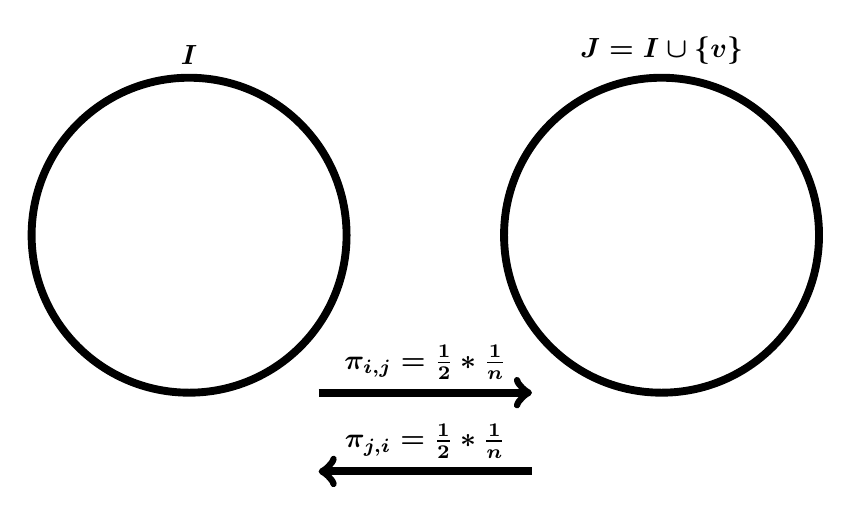
\begin{tikzpicture}[font=\boldmath,ultra thick,]
\draw[solid, line width=1mm]  (0,0) ellipse (2 and 2) node [above=2cm] {$I$};
\draw[solid, line width=1mm]  (6,0) ellipse (2 and 2) node [above=2cm] {$J=I\cup \{v\}$};
\node (v1) at (1.5,-2) {};
\node (v2) at (4.5,-2) {};
\node (v3) at (1.5,-3) {};
\node (v4) at (4.5,-3) {};
\draw[->,solid,line width=1mm,fill=black]  (v1) edge node [above] {$\pi _{i,j}=\frac{1}{2}*\frac{1}{n}$} (v2);
\draw[->,solid,line width=1mm,fill=black]  (v4) edge node [above] {$\pi _{j,i}=\frac{1}{2}*\frac{1}{n}$}(v3);
\end{tikzpicture}
\caption*{$\frac{1}{n}$ $\rightarrow$ wybranie 1 z $n$ wierzchołków\\$\frac{1}{2}$ $\rightarrow$ \textbf{O}rzeł albo \textbf{R}eszka}
\end{figure}
\begin{remark}
Jedynym rozkładem stacjonarnym tego Łańcucha Markowa jest rozkład jednostajny.
\end{remark}
\begin{problem*}
Skonstruować Łańcuch Markowa taki, żeby prawdopodobieństwo każdego ze zbioru niezależnych $I$ było proporcjonalne do $$\alpha ^I$$ gdzie $\alpha $ jest pewną stałą.
\end{problem*}

\subsubsection{Modyfikacja algorytmu}
\begin{enumerate}
\item Startujemy od zbioru pustego $I=\emptyset $
\item Rzucamy monetą taką, że $\mathsf{Pr}(O)=p$\footnote{prawdopodobieństwo ,,wylosowania'' \textbf{O}rła} a $\mathsf{Pr}(R)=1-\mathsf{Pr}(O)=1-p$\footnote{prawdopodobieństwo ,,wylosowania'' \textbf{R}eszki}
\item Wybieramy losowo wierzchołek $v$ w grafie $G$,
\item Jeśli 
\begin{itemize}
\item[] wypadł \textbf{O}rzeł i $I=I\cup \{v\}$ jest niezależny to\\
$I:=I\cup \{v\}$
\item[] wypadła \textbf{R}eszka i $v\in I$ to\\
$I:=I- \{v\}$
\end{itemize}
\item wracamy do punktu 2.
\end{enumerate}

\begin{align*}
\alpha ^{|I|}\pi_{i,j}&=\alpha ^{|J|}\pi_{j,i}\\
\alpha ^{|I|}p\frac{1}{n}=\alpha ^{|J|}(1-p)\frac{1}{n}&=\alpha *\alpha ^{|I|}(1-p)\frac{1}{n}\\
p&=\alpha (1-p)\\
p&=\alpha -\alpha p\\
p+\alpha p&=\alpha\\
p&=\frac{\alpha}{1+\alpha}
\end{align*}

\begin{hipoterm}[Metatwierdzenie (Obserwacja)]
Jeśli potrafimy wygenerować losowy obiekt z danej klasy (być w możę w przybliżeniu) to potrafimy te obiekty (z grubsza) policzyć
\end{hipoterm}

\begin{problem*}
Policz zbiory niezależne w danym grafie $G$
\begin{enumerate}
\item Mamy graf $G$
\item Wybieramy dowolny wierzchołek $v\in V(G)$
\item Szacujemy prawdopodobieństwo $p_v$, że $v$ należy do niezależnego, to znaczy że $v$ należy do $\mathsf{pr}|S_G|$ zbiorów niezależnych \
\item Gdzie $S_G$ jest rodziną wszystkich zbiorów niezależnych w $G$
\begin{enumerate}[label=\Alph*)]
\item Jeśli $p_v\geq \frac{1}{2}$ wtedy $$G'=G- \{v\}-N(v)$$ wtedy $\mathsf{pr}|S_G|-|S_{G'}|$ wybieramy $v'\in V(G')$ i powtarzamy całą procedurę
\item Jeśli $p_v < \frac{1}{2}$ wtedy $$G'=G- \{v\}$$ wybieramy $v'\in V(G')$ i powtarzamy całą procedurę wtedy $$(1-p_v)|S_G|=|S_{G'}|$$
\end{enumerate}
\end{enumerate}
$$\underset{A}{p_{v_1}},\underset{B}{p_{v_2}},\underset{B}{p_{v_3}},...,\underset{B}{p_{v_n}}$$
\begin{figure}[H]
\centering
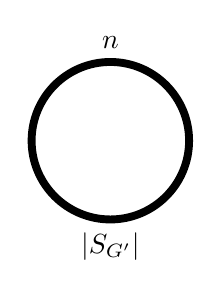
\begin{tikzpicture}
\draw[solid, line width=1mm]  (0,0) ellipse (1 and 1) node [above=1cm] {$n$}
													  node [below=1cm] {$|S_{G'}|$};
\end{tikzpicture}
\end{figure}
\begin{align*}
(1-p_{v_n})|S_{G_{n-1}}|&=|S_{G_n}|\\
|S_{G_{n-1}}|&=\frac{|S_{G_n}|}{1-p_{v_n}}\\
|S_{G_n}|&=\frac{|S_{G_n}|}{\prod_{i=i}^{n-1}\rho _i}\\
\rho _i &= \left\{\begin{matrix}
p_i & \text{ gry zawarte w } A\\
1-p_i &  \text{ gry zawarte w } B
\end{matrix}\right.\\
v_1\ p_{v_1}\geq \frac{1}{2}\ &\ G_2=\{v_1\}\cup N(v_1)\\
v_2\ p_{v_2}\frac{1}{2}\ &\ G_3=g_2- \{v_2\}\\
(1-p_{v_2})|S_{G_2}|&=|S_{G_3}|\\
|S_{G_2}|=\frac{|S_{G_3}|}{1-p_{v_2}}\\
p_{v_1}|S_{G_1}|=|S_{G_2}|&=\frac{|S_{G_3}|}{1-p_{v_2}}\\
|S_{G_1}|&=\frac{|S_{G_3}|}{p_{v_1}(1-p_{v_2})}
\end{align*}
\end{problem*}

